% =====================================================================
% Comparative Analysis of Numerical Interpolation Methods
% for Robot Trajectory Planning
%
% Author: Param Chokshi
% Course: CISC 601 Scientific Computing 2
% Textbook: Chapra & Canale, Numerical Methods for Engineers (8th ed.)
%
% Formatted for the IEEE Transactions / Journals template
% (IEEEtran.cls, journal mode, two-column).
% =====================================================================
\documentclass[journal]{IEEEtran}

% ----- Packages -------------------------------------------------------
\usepackage[utf8]{inputenc}
\usepackage[T1]{fontenc}
\usepackage{lmodern}
\usepackage{microtype}
\usepackage{amsmath, amssymb, amsthm}
\usepackage{graphicx}
\usepackage{booktabs}
\usepackage{array}
\usepackage{tabularx}
\usepackage{caption}
\usepackage{subcaption}
\usepackage{xcolor}
\usepackage{enumitem}
\usepackage{listings}
\usepackage{siunitx}
\usepackage{url}
\usepackage[hidelinks]{hyperref}
\usepackage[capitalize, noabbrev]{cleveref}

% IEEEtran requires hyperref/cleveref to be loaded last and likes
% bookmarks=true. Already loaded above.

% ----- Figure path ----------------------------------------------------
\graphicspath{{figures/}}

% ----- Code listing style --------------------------------------------
\lstset{
    basicstyle=\ttfamily\footnotesize,
    breaklines=true,
    frame=single,
    numbers=left,
    numberstyle=\tiny,
    showstringspaces=false,
}

% ----- Custom commands ------------------------------------------------
% amsmath provides \eqref already; we keep its default behaviour.
\renewcommand{\vec}[1]{\mathbf{#1}}

% =====================================================================
\begin{document}
% =====================================================================

% ----- Title block (IEEEtran style) -----------------------------------
\title{Comparative Analysis of Numerical Interpolation Methods\\
       for Robot Trajectory Planning}

\author{Param~Chokshi%
\thanks{Manuscript submitted \today.
This work was prepared as Deliverable~3 of the research project
for CISC~601 Scientific Computing~2.}%
\thanks{P. Chokshi is a student in CISC~601 Scientific Computing~2
(e-mail: pchokshi@my.harrisburgu.edu).}}

% Header and footer information for journal mode.
\markboth{CISC~601 Scientific Computing~2, Research Project Paper}%
{Chokshi: Comparative Analysis of Numerical Interpolation Methods}

\maketitle

% =====================================================================
% Abstract (IEEEtran format)
% =====================================================================
\begin{abstract}
Robot motion planning routinely produces sequences of waypoints that
must be expanded into smooth time-parameterised trajectories before a
controller can execute them. This paper compares four numerical
interpolation methods drawn from Chapters~18 and~24 of Chapra and
Canale---linear interpolation, natural cubic splines, $C^4$ quintic
splines, and cubic B-spline approximation---under conditions
representative of two industrial robotics scenarios: a two-dimensional
mobile robot navigating an aisle and a two-degree-of-freedom planar
arm performing pick-and-place. Each method is implemented from the
textbook formulation rather than through library black-boxes,
validated against centered finite-difference derivatives
(Chapter~28), and evaluated on seven dataset variants that sweep over
waypoint density (5, 12, 20), geometric character (sharp 90$^{\circ}$
corners versus smooth sinusoid), and time-spacing (chord-length
versus uniform). The results challenge two pieces of conventional
wisdom: increasing waypoint density \emph{worsens} smoothness metrics
under chord-length parameterisation, and the natural-boundary quintic
spline produces \emph{higher} peak acceleration and root-mean-square
jerk than the cubic spline---an artefact entirely attributable to
the boundary condition rather than to the method, since cubic-derived
clamped boundary conditions reduce peak acceleration by 33\% and RMS
jerk by 64\%. The B-spline approximation produces the smoothest
derivatives at the cost of guaranteed waypoint deviation. We provide
a reusable Python implementation, an executable Jupyter notebook,
and a public dataset to support reproducibility.
\end{abstract}

\begin{IEEEkeywords}
B-splines, boundary conditions, cubic splines, finite differences,
interpolation, jerk minimisation, numerical methods, quintic splines,
robotics, trajectory planning, waypoint navigation.
\end{IEEEkeywords}


% =====================================================================
% Introduction
% =====================================================================
\section{Introduction}
\label{sec:introduction}

\IEEEPARstart{M}{odern} robotic systems---from industrial
manipulators on factory floors to autonomous mobile robots in
warehouses---share a fundamental computational challenge: given a
sequence of desired positions (waypoints) produced by a higher-level
path planner, how should the robot interpolate between those
positions to produce motion that is physically feasible, smooth, and
efficient? This question sits at the intersection of numerical
analysis and robotics engineering, and the choice of interpolation
method has direct consequences for mechanical wear, energy
consumption, payload stability, and whether the planned trajectory
can be executed in real time~\cite{biagiotti2008}.

The simplest answer---connecting consecutive waypoints with
straight-line segments---creates abrupt velocity changes at every
waypoint that would require infinite acceleration to follow exactly,
making the trajectory physically infeasible. More sophisticated
interpolation methods from Chapters~18, 24, and 28 of Chapra and
Canale~\cite{chapra2021} address this problem by producing curves
with guaranteed continuity in velocity, acceleration, or even jerk
(the time derivative of acceleration). Higher-order continuity
generally reduces the mechanical disturbance that the robot
experiences during motion, but every additional constraint must be
paid for somewhere, and the practical trade-offs are not always
obvious from the asymptotic analysis alone.

\subsection{Problem statement}
\label{sec:problem-statement}

A robot is given a sequence of $n+1$ waypoints
$\{(t_i, \vec{p}_i)\}_{i=0}^{n}$ where $\vec{p}_i \in \mathbb{R}^d$ is
the desired configuration at time $t_i$. We require an interpolating
function $\vec{p}(t) : [t_0, t_n] \to \mathbb{R}^d$ such that
$\vec{p}(t_i) = \vec{p}_i$ (or, in the case of approximation methods,
$\vec{p}(t_i) \approx \vec{p}_i$). The choice of $\vec{p}(\cdot)$
should be evaluated against multiple criteria: positional accuracy,
velocity continuity, acceleration smoothness, jerk minimisation,
computational cost, and total path length.

The central question this paper addresses is:

\begin{quote}
\itshape Among the numerical interpolation methods presented in
Chapters~18 and~24 of Chapra and Canale, which produces the most
suitable trajectories for robotic applications, and under what
conditions does each method excel or fail?
\end{quote}

\subsection{Contributions}
\label{sec:contributions}

This paper makes the following contributions:

\begin{enumerate}[leftmargin=*]
\item We provide textbook-formulation Python implementations of four
interpolation methods---linear (Eq.~18.2 of \cite{chapra2021}),
natural and clamped cubic splines (Eq.~18.36--18.37), $C^4$ quintic
Hermite splines, and cubic B-spline approximation via the Cox--de
Boor recursion---validated against reference implementations and
analytic test functions.
\item We construct two robotics datasets (a 12-waypoint mobile-robot
aisle and an 8-waypoint 2-DOF arm pick-and-place) and seven dataset
variants that sweep over waypoint density, geometric character, and
time spacing.
\item We evaluate each method under each variant against six
quantitative metrics (peak speed, peak acceleration, RMS jerk, total
path length, maximum waypoint error, computation time) and a seventh
that quantifies $C^1$ violations directly.
\item We validate the analytic derivative formulas against
finite-difference numerical derivatives drawn from Chapter~28 of
\cite{chapra2021}, confirming agreement to better than $10^{-3}$ in
the relevant units.
\item We identify a non-obvious result: the quintic spline's
apparently inferior smoothness under natural boundary conditions is
an artefact of the boundary condition itself, not the method;
cubic-derived clamped boundary conditions recover and exceed the
cubic spline's performance.
\end{enumerate}

\subsection{Paper organisation}

The remainder of the paper is organised as follows.
Section~\ref{sec:background} reviews the relevant numerical methods
and the robotics-specific motivation for studying them.
Section~\ref{sec:methodology} describes the implementation, the
datasets, and the evaluation metrics. Section~\ref{sec:results}
presents quantitative results from the baseline scenarios, the full
variant sweep, the derivative validation, and the boundary-condition
sensitivity study. Section~\ref{sec:discussion} interprets the
findings in the context of practical trajectory generation, and
Section~\ref{sec:conclusion} concludes with limitations and future
work.


% =====================================================================
% Background
% =====================================================================
\section{Background}
\label{sec:background}

\subsection{Continuity classes and their physical meaning}
\label{sec:continuity}

A trajectory $\vec{p}(t)$ is said to belong to continuity class $C^k$
on its domain if $\vec{p}$ together with all derivatives up to order
$k$ exist and are continuous. The lowest non-trivial class, $C^0$,
requires only that position be continuous; the higher classes $C^1$,
$C^2$, $C^3$, $C^4$ progressively add velocity, acceleration, jerk,
and snap. Each class corresponds to a directly-observable physical
property:

\begin{itemize}[leftmargin=*]
\item A trajectory that fails $C^1$ has a velocity jump somewhere
along its domain. To track such a trajectory exactly, an actuator
would need to apply infinite force for an instant, which is not
physically realisable.
\item A trajectory that fails $C^2$ has discontinuous acceleration,
which a real actuator can approximate but only by demanding step
changes in motor torque. This induces measurable vibration in the
mechanical structure~\cite{macfarlane2003jerk}.
\item A trajectory that fails $C^3$ has discontinuous jerk. Because
inertial loads with compliant mounts respond at finite bandwidth,
discontinuous jerk excites mechanical resonances and makes payloads
slosh or shift~\cite{kyriakopoulos1988minimum}.
\end{itemize}

The four interpolation methods in this study span the relevant
continuity classes (\cref{tab:continuity-classes}).

\begin{table}[!t]
\centering
\caption{Continuity properties of the four interpolation methods
studied. Linear interpolation is $C^0$; cubic and quintic splines
are $C^2$ and $C^4$ respectively; the cubic B-spline is $C^2$
across the entire curve.}
\label{tab:continuity-classes}
\begin{tabularx}{\linewidth}{lcX}
\toprule
\textbf{Method} & \textbf{Continuity} & \textbf{Waypoint behaviour} \\
\midrule
Linear (Eq.~18.2 of \cite{chapra2021})         & $C^0$ & Passes through every waypoint \\
Cubic spline (Eq.~18.36)                       & $C^2$ & Passes through every waypoint \\
Quintic spline (Hermite construction)          & $C^4$ & Passes through every waypoint \\
Cubic B-spline (Cox--de Boor) \cite{piegl1997nurbs} & $C^2$ & Passes through endpoints only (clamped knot vector); approximates interior \\
\bottomrule
\end{tabularx}
\end{table}

\subsection{Linear interpolation}
\label{sec:bg-linear}

Linear interpolation between two consecutive waypoints
$(t_i, \vec{p}_i)$ and $(t_{i+1}, \vec{p}_{i+1})$ is given
by~\cite[Eq.~18.2]{chapra2021}
\begin{equation}
\vec{p}(t) = \vec{p}_i + \frac{\vec{p}_{i+1} - \vec{p}_i}{t_{i+1} - t_i}
             (t - t_i), \quad t \in [t_i, t_{i+1}].
\label{eq:linear}
\end{equation}
The resulting curve is $C^0$ but not $C^1$: the derivative $\dot{\vec{p}}(t)$
is piecewise constant with a step change at each interior knot.
Higher derivatives are zero everywhere on the open intervals; in the
distributional sense, $\ddot{\vec{p}}(t)$ contains Dirac impulses at
every waypoint.

\subsection{Cubic spline interpolation}
\label{sec:bg-cubic}

A cubic spline is a piecewise cubic polynomial interpolant that is
$C^2$ across the entire knot sequence. Following \cite[Section
18.6]{chapra2021}, we let $M_i = \ddot{\vec{p}}(t_i)$ and write each
segment in the closed form
\begin{align}
\vec{p}_i(t) &= \frac{M_i}{6 h_i}(t_{i+1} - t)^3
              + \frac{M_{i+1}}{6 h_i}(t - t_i)^3 \nonumber\\
            &+ \left(\frac{\vec{p}_i}{h_i} - \frac{M_i h_i}{6}\right)(t_{i+1} - t)
              \nonumber\\
            &+ \left(\frac{\vec{p}_{i+1}}{h_i} - \frac{M_{i+1} h_i}{6}\right)(t - t_i),
\label{eq:cubic-segment}
\end{align}
where $h_i = t_{i+1} - t_i$. Imposing $C^1$ continuity at every
interior knot produces the tridiagonal system
\cite[Eq.~18.37]{chapra2021}
\begin{equation}
h_{i-1} M_{i-1} + 2(h_{i-1} + h_i) M_i + h_i M_{i+1} = R_i,
\label{eq:cubic-system}
\end{equation}
with right-hand side
$R_i = 6/h_i (\vec{p}_{i+1} - \vec{p}_i)
     - 6/h_{i-1} (\vec{p}_i - \vec{p}_{i-1})$
for $i = 1, \dots, n-1$. Two boundary equations close the system; we
use the natural boundary $M_0 = M_n = \vec{0}$ throughout this paper
unless otherwise stated.

\subsection{Quintic spline interpolation}
\label{sec:bg-quintic}

A quintic spline extends the cubic construction to fifth-degree
polynomials with $C^4$ continuity across knots. We parameterise each
segment using the unit-interval variable $s = (t - t_i)/h_i$ and
write
\begin{align}
\vec{p}_i(s) &= H_0(s) \vec{p}_i + H_1(s) h_i \vec{v}_i + H_2(s) h_i^2 \vec{a}_i \nonumber\\
           &\quad + H_3(s) \vec{p}_{i+1} + H_4(s) h_i \vec{v}_{i+1}
                 + H_5(s) h_i^2 \vec{a}_{i+1},
\label{eq:quintic-hermite}
\end{align}
where $H_0,\dots,H_5$ are the standard quintic Hermite basis functions
and the unknowns are the velocity $\vec{v}_i$ and acceleration
$\vec{a}_i$ at each knot. Position, velocity, and acceleration are
continuous by construction; continuity of the third and fourth time
derivatives at internal knots provides $2(n-1)$ linear equations in
the $2(n+1)$ unknowns, which we close with four boundary equations.
The natural boundary condition sets
$\vec{v}_0 = \vec{a}_0 = \vec{v}_n = \vec{a}_n = \vec{0}$
(start and stop at rest in both velocity and acceleration); the
clamped variant lets the user specify these four quantities directly.

\subsection{Cubic B-spline approximation}
\label{sec:bg-bspline}

A B-spline curve of degree $p$ with knot vector $T = (t_0, \dots, t_m)$
and control points $\vec{P}_0, \dots, \vec{P}_{m-p-1}$ is defined by
\begin{equation}
\vec{C}(t) = \sum_{i=0}^{m-p-1} N_{i,p}(t) \vec{P}_i,
\label{eq:bspline-curve}
\end{equation}
where the basis functions $N_{i,p}$ are computed by the Cox--de Boor
recursion~\cite{piegl1997nurbs, deboor1978}:
\begin{align}
N_{i,0}(t) &= \begin{cases} 1 & t_i \le t < t_{i+1}, \\ 0 & \text{otherwise}, \end{cases}\\
N_{i,p}(t) &= \frac{t - t_i}{t_{i+p} - t_i} N_{i,p-1}(t)
            + \frac{t_{i+p+1} - t}{t_{i+p+1} - t_{i+1}} N_{i+1,p-1}(t).
\label{eq:cox-de-boor}
\end{align}
We use a cubic B-spline ($p=3$) with a clamped, ``averaged'' knot
vector. The first and last knots are repeated $p+1$ times so that the
curve passes through the first and last waypoint exactly; interior
knots are placed at the average of $p$ consecutive parameter values.
The waypoints serve as control points; the curve approximates the
interior rather than interpolating it, providing the local-control
property and inherent smoothness that distinguish B-splines from
classical splines~\cite{piegl1997nurbs}.

\subsection{Numerical differentiation}
\label{sec:bg-diff}

Following Chapter~28 of \cite{chapra2021}, we use centered
finite-difference formulas to compute velocity, acceleration, and
jerk profiles from sampled trajectories. The five-point centered
formula for the first derivative,
\begin{equation}
f'(x_i) \approx \frac{-f_{i+2} + 8 f_{i+1} - 8 f_{i-1} + f_{i-2}}{12 h},
\label{eq:five-point}
\end{equation}
is $\mathcal{O}(h^4)$ accurate; the three-point centered formula for
the second derivative,
\begin{equation}
f''(x_i) \approx \frac{f_{i+1} - 2 f_i + f_{i-1}}{h^2},
\label{eq:three-point-second}
\end{equation}
is $\mathcal{O}(h^2)$. These formulas are used in
Section~\ref{sec:results} to validate that our analytic derivative
implementations agree with the textbook finite differences.

\subsection{Robotics context}

Trajectory planning for robots is the process of converting a
geometric path (a sequence of poses or waypoints) into a
time-parameterised motion plan that the controller can
execute~\cite{biagiotti2008, siciliano2009}. Mobile robots and robot
manipulators differ in the natural choice of configuration space:
mobile-robot waypoints are typically Cartesian $(x, y)$ poses,
whereas manipulator waypoints are joint-angle vectors related to
end-effector poses through nonlinear forward
kinematics~\cite{craig2018}. The two scenarios in this paper
exercise both modes.


% =====================================================================
% Methodology
% =====================================================================
\section{Methodology}
\label{sec:methodology}

\subsection{Implementation overview}
\label{sec:impl-overview}

All four interpolation methods were implemented in Python~3.12 using
NumPy~\cite{numpy} and SciPy~\cite{scipy}. As the proposal required,
each method was coded directly from the textbook formulation rather
than wrapping a library black-box. SciPy was used only as a numerical
linear-algebra back-end---specifically \texttt{scipy.linalg.solve\_banded}
for the cubic-spline tridiagonal system and \texttt{scipy.linalg.solve}
for the quintic-spline dense system. The B-spline basis was built via
the Cox--de Boor recursion (Equation~\ref{eq:cox-de-boor}) without
relying on \texttt{scipy.interpolate.BSpline}. The complete source
code, datasets, and results are available in the project repository.

The cubic and B-spline implementations were validated against
SciPy's reference \texttt{CubicSpline} and \texttt{BSpline} classes
on identical inputs and agreed to machine precision (maximum error
$\sim 10^{-15}$). The quintic-spline implementation was validated by
reconstructing a known fifth-degree polynomial; the implementation
reproduced both the polynomial values and its analytic derivatives
to floating-point precision ($\sim 10^{-13}$).

\subsection{Datasets}
\label{sec:datasets}

\subsubsection{Mobile robot scenario.}
The mobile-robot dataset consists of twelve $(x, y)$ waypoints in
metres representing a robot navigating a warehouse aisle. The path
includes a straight entry segment, a sharp 90$^{\circ}$ right turn
around a shelving unit, a diagonal traverse to a pick station, a
90$^{\circ}$ left turn back into the main aisle, and a gentle
S-curve to the exit. Waypoint times use chord-length parameterisation
at a nominal speed of 1\,m/s, the standard recommendation in
\cite[Section 24.1]{chapra2021} for non-uniformly spaced data. Total
trajectory time is 24.93\,s.

\subsubsection{Robot arm scenario.}
The robot-arm dataset describes a 2-DOF planar manipulator with link
lengths $L_1 = \SI{0.5}{\meter}$ and $L_2 = \SI{0.4}{\meter}$
performing a pick-and-place cycle. The cycle visits eight joint-space
waypoints (in degrees, converted to radians internally): home,
approach over part, grasp, lift, transfer mid-point, over placement
bay, place, retract. Forward kinematics maps joint angles to
Cartesian end-effector position via
\begin{align}
x &= L_1 \cos\theta_1 + L_2 \cos(\theta_1 + \theta_2),\\
y &= L_1 \sin\theta_1 + L_2 \sin(\theta_1 + \theta_2),
\end{align}
following Chapter~3 of \cite{craig2018}. All Cartesian waypoints lie
within the reachable workspace $\|(x,y)\| \le L_1 + L_2 = \SI{0.9}{\meter}$.
Waypoint timing is uniform at one second per segment for a total of
seven seconds.

\subsubsection{Variant datasets for the experimental sweep.}
To investigate how each method's behaviour depends on input
characteristics, we generated five additional dataset variants by
sweeping over three independent axes: waypoint density, geometric
character, and time spacing
(\cref{tab:variant-summary}). The variant family is designed so that
each axis varies in isolation: the density sweep holds geometry and
spacing fixed, the geometry sweep holds density and spacing fixed,
and the spacing sweep holds geometry and density fixed.

\begin{table}[!t]
\centering
\caption{Dataset variants used in the experimental sweep. The
canonical baseline is \texttt{mixed\_baseline\_chord}; each row
varies exactly one axis from the baseline.}
\label{tab:variant-summary}
\begin{tabular}{lccc}
\toprule
\textbf{Variant} & \textbf{Geometry} & \textbf{Spacing} & \textbf{$n$} \\
\midrule
mixed\_sparse\_chord       & mixed   & chord   &  5 \\
mixed\_baseline\_chord     & mixed   & chord   & 12 \\
mixed\_dense\_chord        & mixed   & chord   & 20 \\
sharp\_n12\_chord          & sharp   & chord   & 12 \\
gradual\_n12\_chord        & gradual & chord   & 12 \\
mixed\_baseline\_uniform   & mixed   & uniform & 12 \\
robot\_arm\_baseline       & arm     & uniform &  8 \\
\bottomrule
\end{tabular}
\end{table}

The geometry options are: a \emph{mixed} warehouse-aisle path
(arc-length resampled from the original 12-vertex polyline at the
desired density); a \emph{sharp} rectangular zigzag with eleven
segments alternating between horizontal and vertical and exact 90$^{\circ}$
interior corners; and a \emph{gradual} sinusoidal path
$y = A \sin(2\pi k x / X)$ chosen so every method should agree
closely. The spacing options are chord-length parameterisation and
uniform time spacing.

\subsection{Evaluation metrics}
\label{sec:metrics}

We evaluate each method-dataset pairing using the metrics summarised
in \cref{tab:metrics}. Apart from \texttt{compute\_time\_ms} and the
positional accuracy measure \texttt{max\_waypoint\_err}, all metrics
are computed from a dense sample of 1000 evenly spaced points
generated by analytic evaluation of the interpolant.

\begin{table}[!t]
\centering
\caption{Quantitative evaluation metrics. Norms are Euclidean.}
\label{tab:metrics}
\begin{tabularx}{\linewidth}{lX}
\toprule
\textbf{Metric}     & \textbf{Definition} \\
\midrule
\texttt{max\_speed}    & $\max_t \| \dot{\vec{p}}(t) \|$ \\
\texttt{max\_accel}    & $\max_t \| \ddot{\vec{p}}(t) \|$ \\
\texttt{rms\_jerk}     & $\sqrt{\frac{1}{T} \int_0^T \| \dddot{\vec{p}}(t) \|^2 dt}$
                          (trapezoidal quadrature) \\
\texttt{path\_length}  & $\int_0^T \| \dot{\vec{p}}(t) \|\, dt$
                          (trapezoidal quadrature) \\
\texttt{max\_waypoint\_err} & $\max_i \|\vec{p}(t_i) - \vec{p}_i\|$ \\
\texttt{max\_velocity\_disc} & $\max_i \|\dot{\vec{p}}(t_i^+) - \dot{\vec{p}}(t_i^-)\|$
                                (probe with $\varepsilon = 10^{-6}(t_n - t_0)$) \\
\texttt{compute\_time\_ms}   & wall-clock time to construct and densely
                                evaluate the interpolant \\
\bottomrule
\end{tabularx}
\end{table}

The \texttt{max\_velocity\_disc} metric provides a direct,
quantitative measure of $C^1$ violation. For a $C^1$ method the
left- and right-limits of the velocity at any internal knot agree,
so the probe returns a value proportional to $2\varepsilon \cdot
\max\|\ddot{\vec{p}}\|$ (essentially numerical noise). For linear
interpolation the limits differ, and the probe returns the actual
magnitude of the velocity jump.

\subsection{Validation methodology}
\label{sec:validation-method}

To verify that the analytic-derivative formulas of each
interpolation method are correctly implemented, we densely sample
each method's position output and compute first, second, and third
derivatives by finite difference using the schemes from
Section~\ref{sec:bg-diff}. We then compare the analytic and empirical
derivatives over the interior of the trajectory (excluding the
boundary regions where finite differences fall back to lower-order
one-sided stencils). Disagreement that scales with $h^k$ for the
expected order of accuracy indicates a correctly-implemented analytic
derivative; disagreement that does not scale with $h$ would indicate
a bug.

\subsection{Boundary-condition sensitivity study}
\label{sec:bc-sensitivity-method}

After observing that the natural-boundary quintic spline produced
unexpectedly large peak acceleration and RMS jerk on the baseline
mobile-robot dataset (Section~\ref{sec:results}), we conducted an
ad-hoc sensitivity study comparing two boundary-condition variants
of the same quintic spline:

\begin{itemize}[leftmargin=*]
\item \textbf{Natural BC}: $\vec{v}_0 = \vec{a}_0 = \vec{v}_n = \vec{a}_n = \vec{0}$.
\item \textbf{Cubic-derived clamped BC}: $\vec{v}_0, \vec{v}_n, \vec{a}_0, \vec{a}_n$
      are read off the cubic-spline solution at the same knots, then
      passed to the quintic spline as clamped boundary values.
\end{itemize}

The sensitivity study quantifies how much of the observed quintic
behaviour is attributable to the boundary condition rather than the
method itself.


% =====================================================================
% Results
% =====================================================================
\section{Results}
\label{sec:results}

\subsection{Baseline scenarios}
\label{sec:results-baseline}

\Cref{fig:mobile-traj} shows the four interpolated trajectories for
the 12-waypoint mobile-robot baseline. Linear interpolation is
identical to the waypoint polygon by construction. The cubic and
quintic splines pass exactly through every waypoint and round the
two 90$^{\circ}$ corners with visibly different tightness. The
B-spline approximation deviates noticeably from the interior
waypoints, cutting both 90$^{\circ}$ corners and producing a
shorter overall path.

\begin{figure}[!t]
\centering
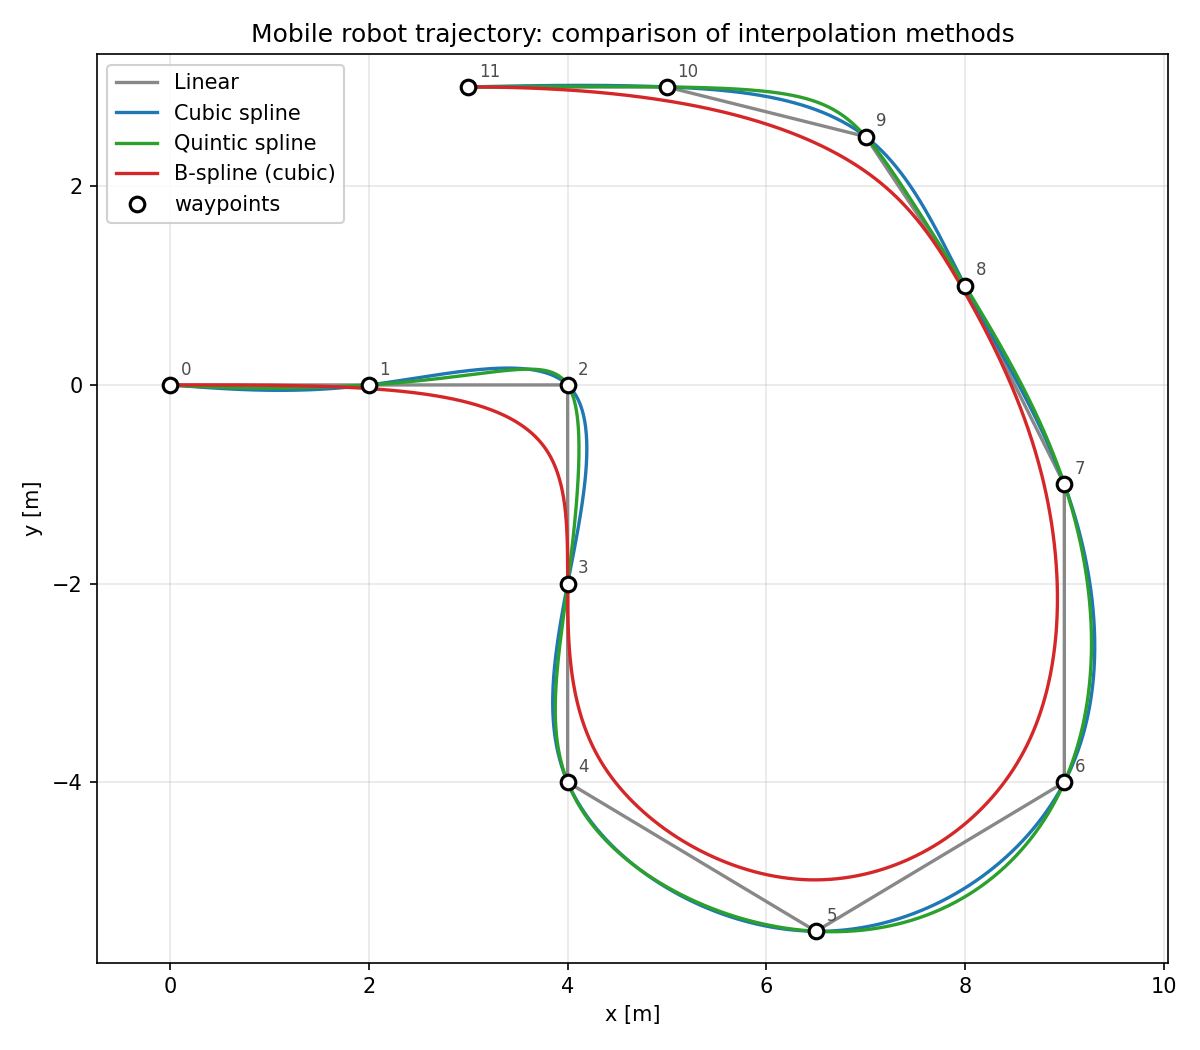
\includegraphics[width=\linewidth]{mobile_robot_trajectory.png}
\caption{Mobile-robot trajectory: comparison of the four
interpolation methods on the 12-waypoint baseline. White circles are
the waypoints; numbered for reference.}
\label{fig:mobile-traj}
\end{figure}

The kinematic profile in \cref{fig:mobile-kinematics} reveals the
qualitative differences between the methods that are not visible from
the trajectory plot alone. Linear interpolation has zero analytic
acceleration and zero analytic jerk because each segment is a
constant-velocity straight line. Cubic spline jerk exhibits the
characteristic step pattern of a piecewise-cubic interpolant whose
third derivative is constant on each segment. Quintic spline jerk is
continuous but has visibly larger amplitude near $t=0$ and $t=T$,
where natural boundary conditions force a rapid transition from rest
to nominal speed. The B-spline produces the smoothest derivative
profile by every metric.

\begin{figure*}[!t]
\centering
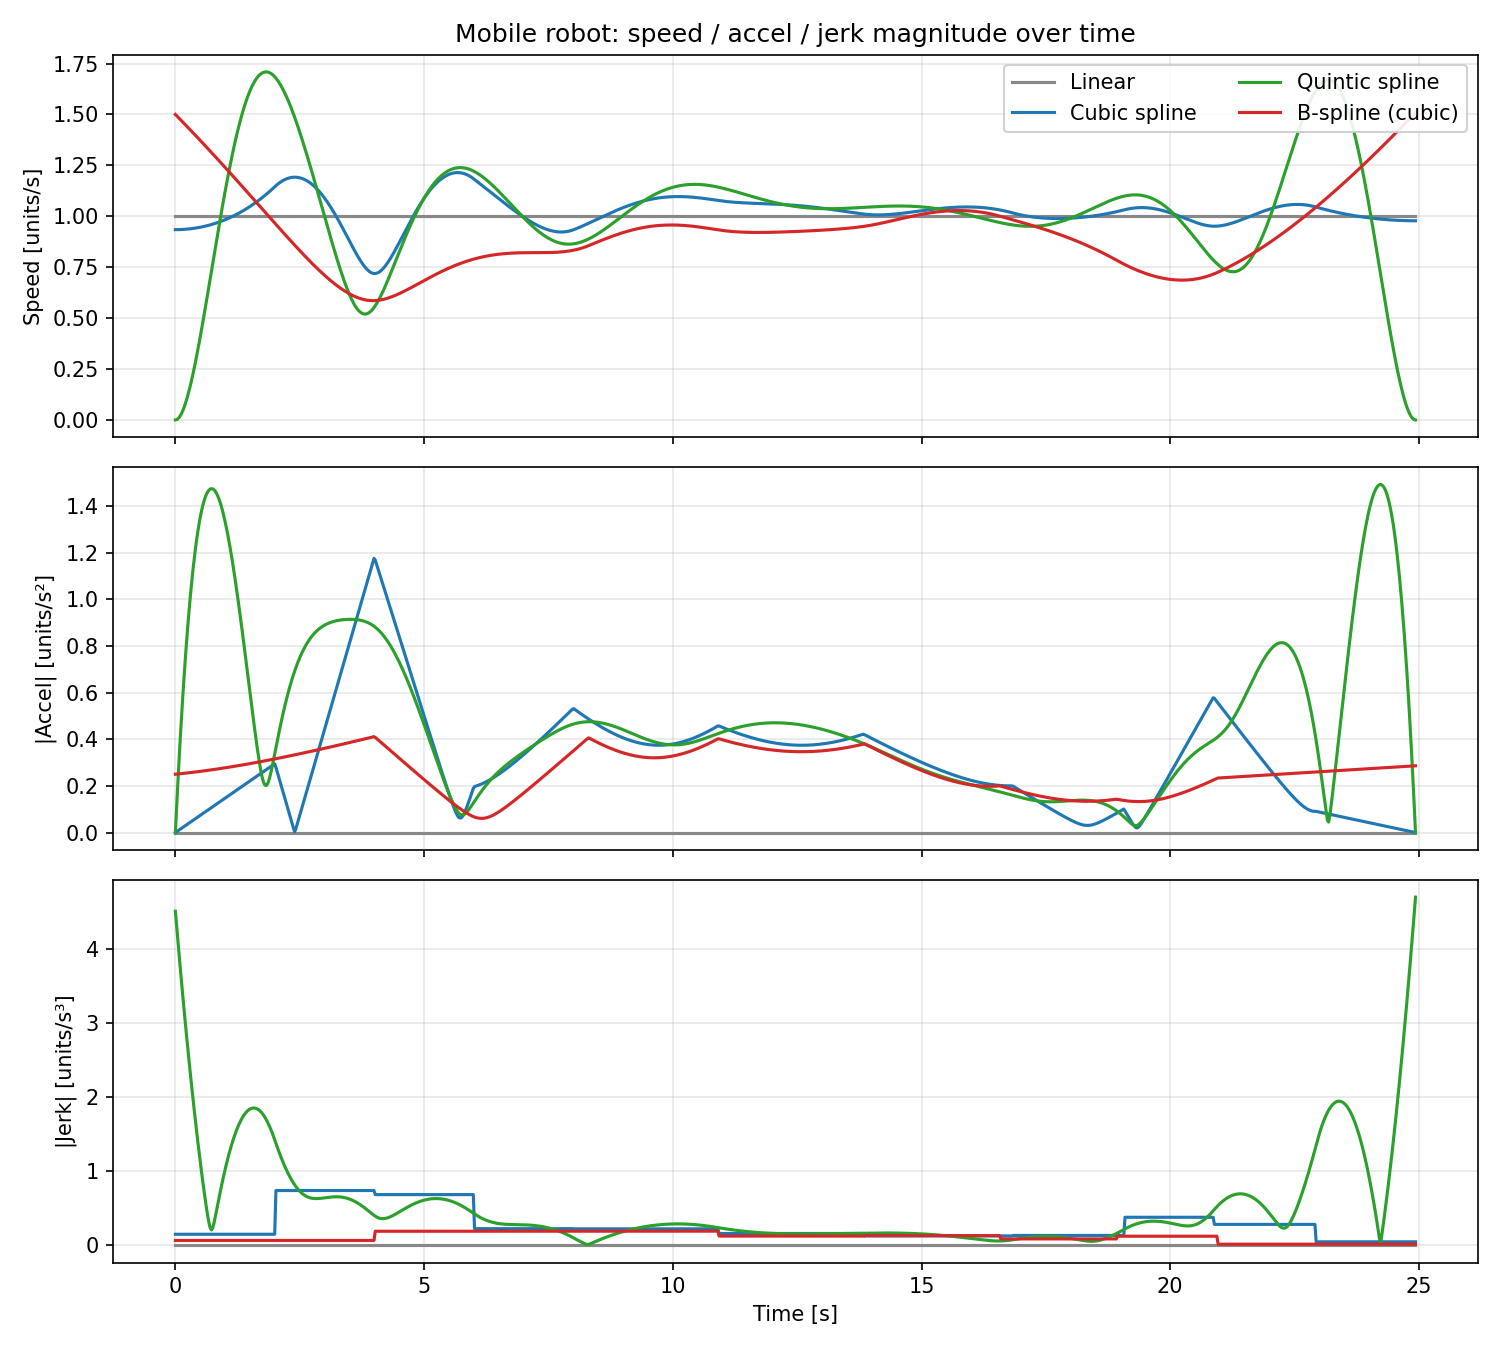
\includegraphics[width=0.78\linewidth]{mobile_robot_kinematics.png}
\caption{Mobile-robot baseline: speed, acceleration magnitude, and
jerk magnitude profiles for each method. Note the piecewise-constant
jerk pattern of the cubic spline and the endpoint jerk spikes of the
natural-BC quintic spline.}
\label{fig:mobile-kinematics}
\end{figure*}

For the robot-arm scenario, \cref{fig:arm-cartesian} shows the
end-effector trajectories produced by mapping each method's
joint-space output through forward kinematics. Even though every
interpolating method visits the same eight joint waypoints, the
Cartesian paths between them differ because the kinematic mapping is
nonlinear. The natural-BC quintic produces visible loops near
waypoints 2 and 5--6 that are not present in the cubic.

\begin{figure}[!t]
\centering
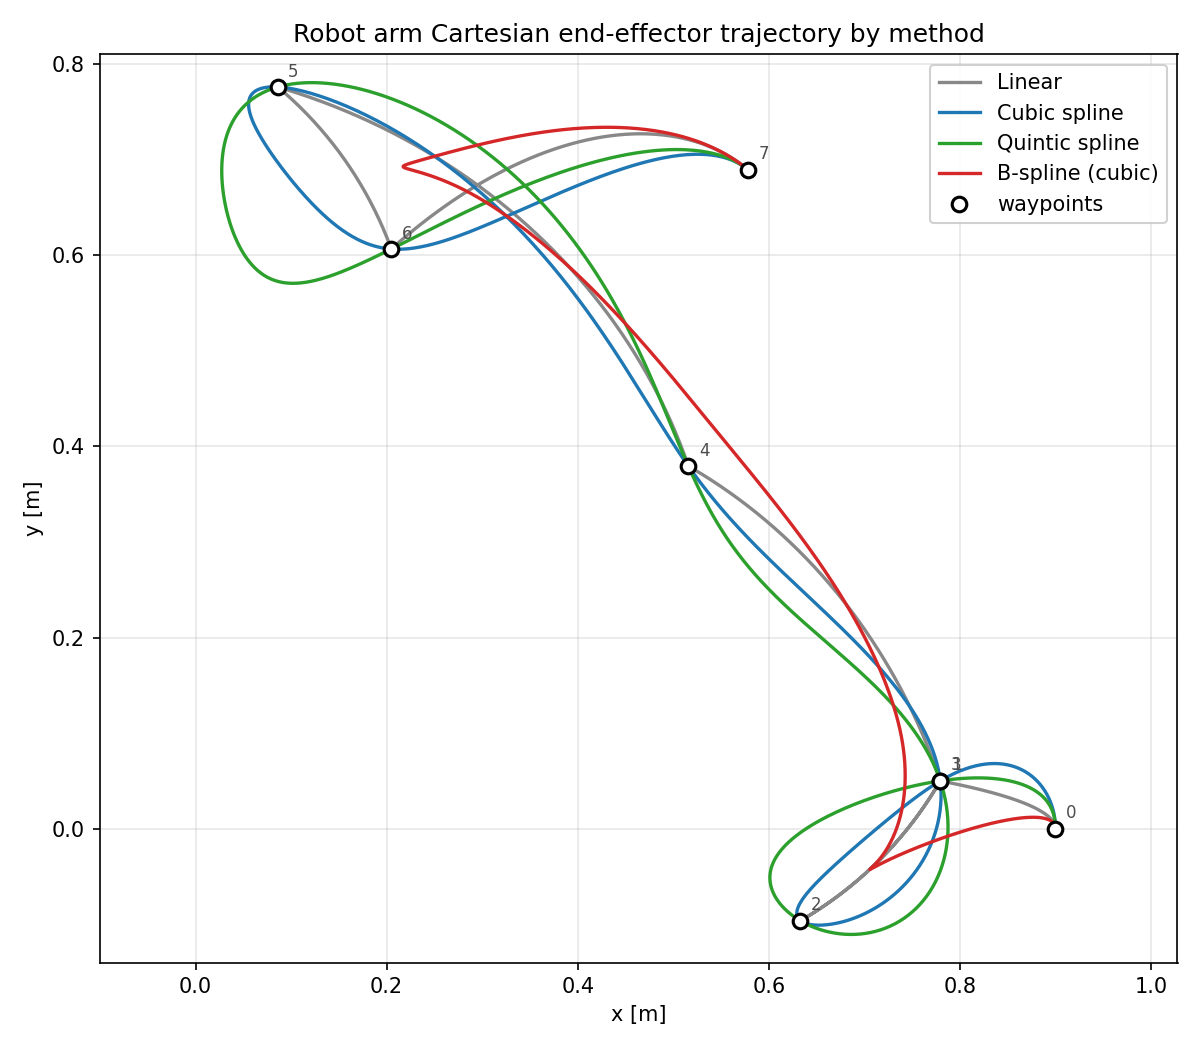
\includegraphics[width=\linewidth]{robot_arm_cartesian.png}
\caption{Robot-arm Cartesian end-effector trajectories: result of
running each method on the joint-space waypoints and projecting
through forward kinematics.}
\label{fig:arm-cartesian}
\end{figure}

\begin{table*}[t]
\centering
\caption{Baseline metrics for all four methods on both scenarios.
Mobile-robot units are metres; arm units are radians for joint-space
quantities. \texttt{wp\_err} is the maximum waypoint deviation;
\texttt{disc} is the maximum velocity discontinuity at internal knots.}
\label{tab:baseline-metrics}
\begin{tabular}{llrrrrrrr}
\toprule
\textbf{Dataset} & \textbf{Method} & $\max\|v\|$ & $\max\|a\|$ & $\mathrm{rms}\|j\|$ & path & wp\_err & disc & $t$ (ms) \\
\midrule
Mobile robot & Linear   & 1.000 & 0.000 & 0.000 & 24.93 & $0$ & $1.41$ & 0.13 \\
             & Cubic    & 1.215 & 1.175 & 0.340 & 25.51 & $0$ & $9{\times}10^{-5}$ & 0.37 \\
             & Quintic  & 1.709 & 1.491 & 0.854 & 25.52 & $0$ & $8{\times}10^{-5}$ & 0.75 \\
             & B-spline & 1.509 & 0.411 & 0.126 & 22.92 & $0.68$ & $3{\times}10^{-5}$ & 0.65 \\
\midrule
Robot arm    & Linear   & 1.888 & 0.000 & 0.000 & 6.37 & $0$ & --- & 0.12 \\
             & Cubic    & 2.580 & 4.225 & 5.191 & 6.66 & $0$ & --- & 0.29 \\
             & Quintic  & 2.958 & 6.810 & 10.986 & 7.63 & $0$ & --- & 0.67 \\
             & B-spline & 2.832 & 3.280 & 1.566 & 4.51 & $0.40$ & --- & 0.44 \\
\bottomrule
\end{tabular}
\end{table*}

The quantitative metrics in \cref{tab:baseline-metrics} confirm
several observations from the figures. The interpolating methods all
hit every waypoint to floating-point precision; only the B-spline
deviates (0.68\,m on the mobile robot, 0.40\,rad on the robot arm).
Linear interpolation reports zero analytic acceleration but a $\sim 1$\,m/s
velocity-discontinuity magnitude on the mobile robot, in contrast to
the smooth methods whose discontinuity values sit at $10^{-5}$\,m/s
and below (the latter is dominated by $\varepsilon$-proportional
numerical noise from the finite-difference probe). Surprisingly, the
quintic spline produces \emph{higher} peak acceleration and RMS jerk
than the cubic on both datasets despite its higher continuity class;
this anomaly is investigated in Section~\ref{sec:results-bc-sens}.

\subsection{Density sweep}
\label{sec:results-density}

\Cref{fig:density-sweep} sweeps over waypoint count
$n \in \{5, 12, 20\}$ on the mixed warehouse-aisle geometry under
chord-length parameterisation. Counter to a naive expectation that
``more waypoints means smoother motion'', peak acceleration and RMS
jerk both increase monotonically with $n$ for every spline-style
method.

\begin{figure*}[!t]
\centering
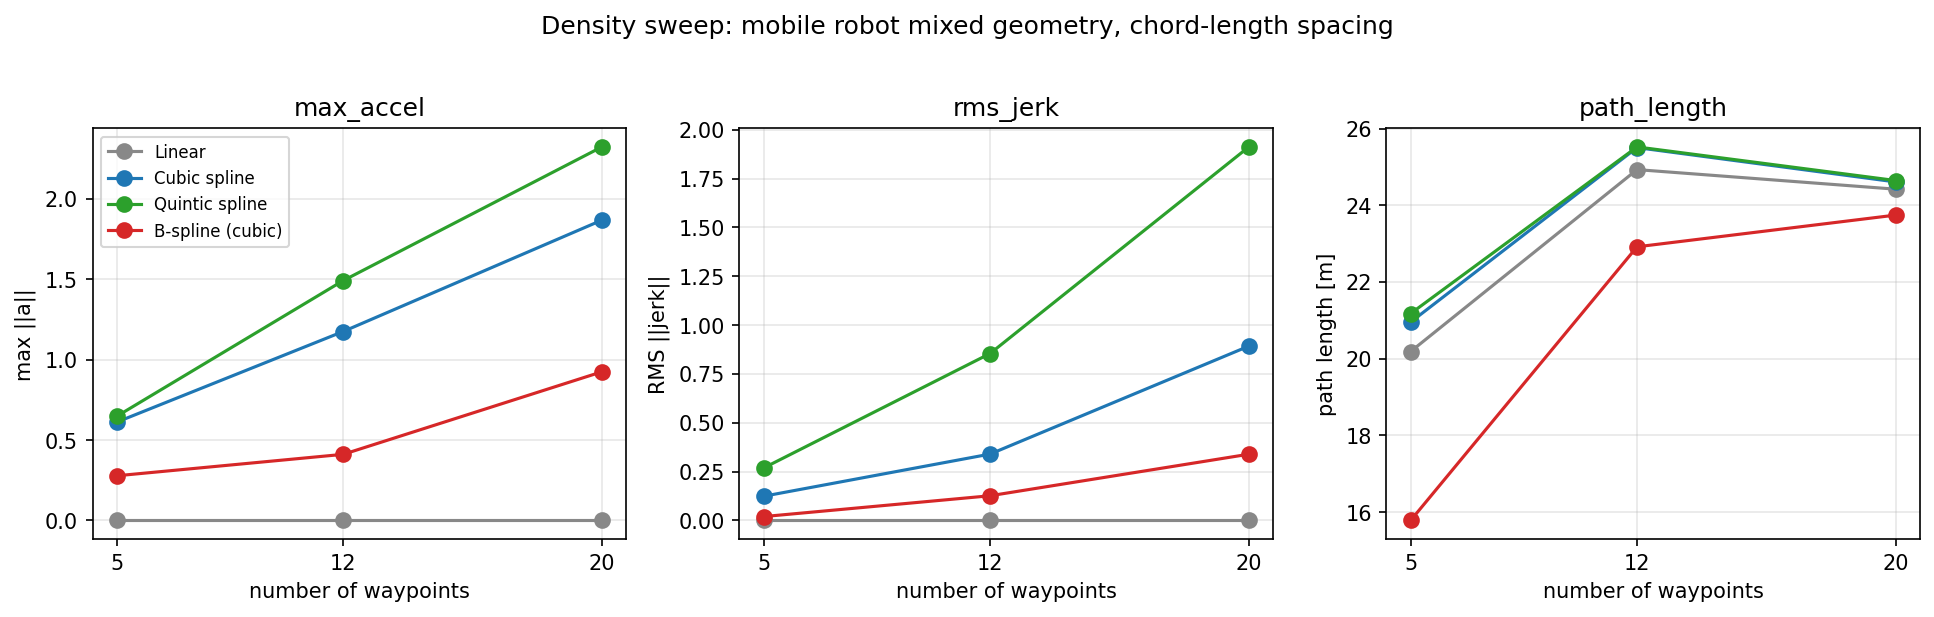
\includegraphics[width=\linewidth]{sweep_density.png}
\caption{Density sweep: peak acceleration, RMS jerk, and path length
versus waypoint count on the mixed mobile-robot geometry with
chord-length spacing. Acceleration and jerk increase monotonically;
path length converges towards the polyline.}
\label{fig:density-sweep}
\end{figure*}

The mechanism is straightforward when viewed alongside the
trajectories themselves (\cref{fig:density-trajectories}): denser
waypoints under chord-length spacing reduce the segment width $h_i$
proportionally, forcing larger curvatures into the splines and
generating proportionally larger time derivatives. Path length
converges towards the polyline as $n$ grows, demonstrating that
geometric fidelity improves while smoothness deteriorates.

\begin{figure*}[!t]
\centering
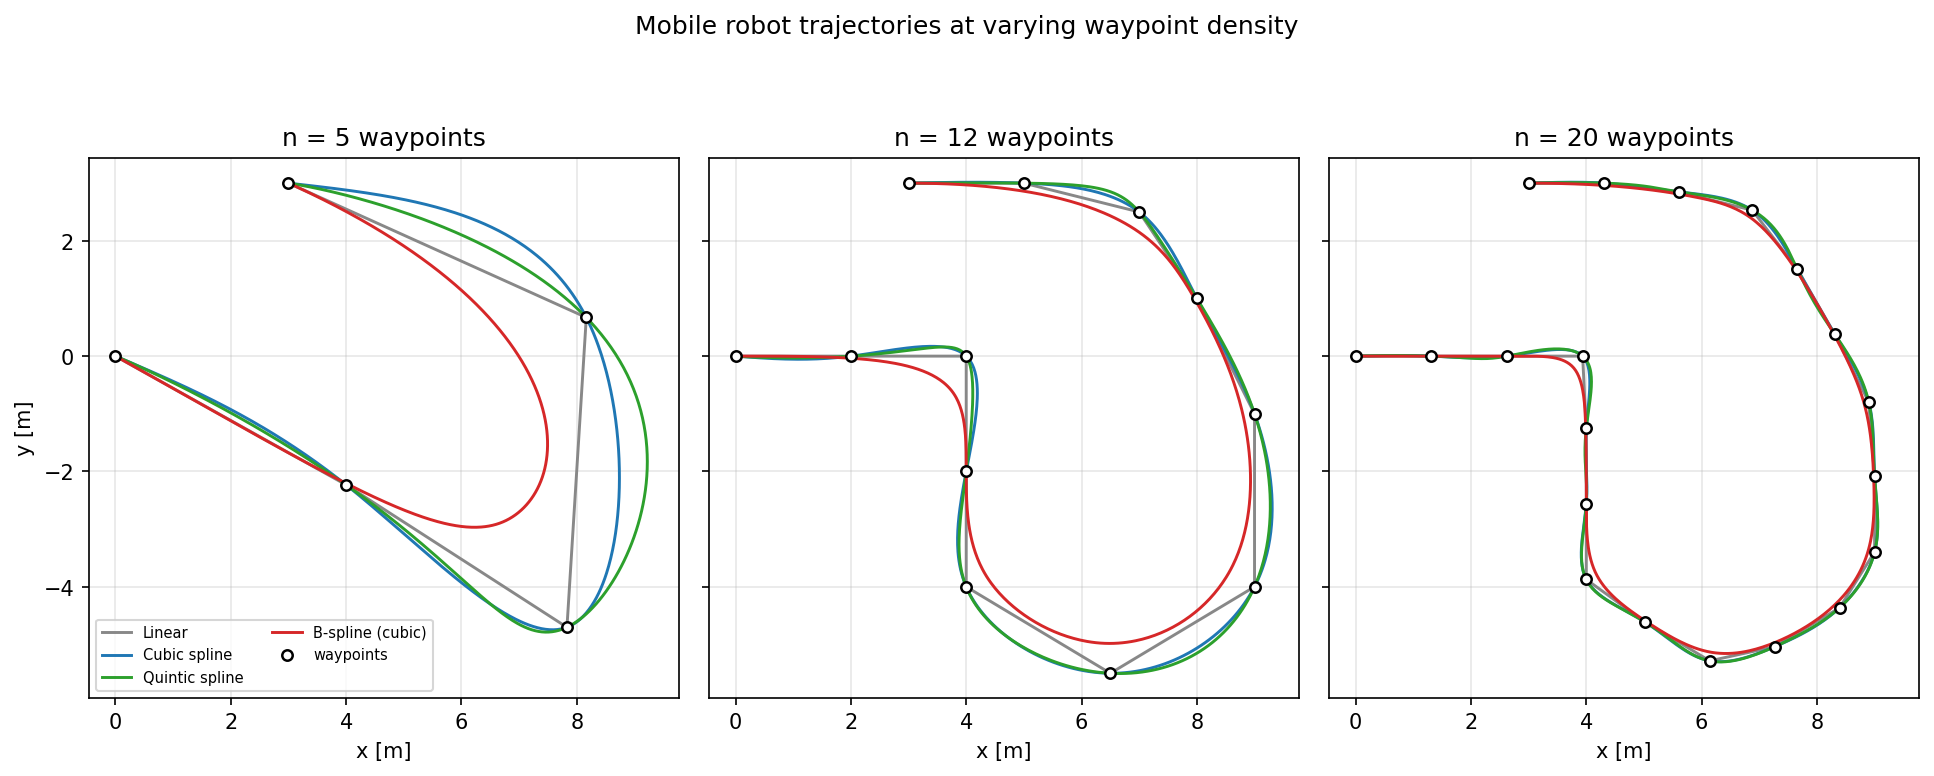
\includegraphics[width=\linewidth]{sweep_density_trajectories.png}
\caption{Mobile-robot trajectories at varying waypoint density. At
$n=5$ all smooth methods make obvious geometric mistakes; at $n=20$
they trace the polyline closely.}
\label{fig:density-trajectories}
\end{figure*}

\subsection{Geometry sweep}
\label{sec:results-geometry}

\Cref{fig:geometry-sweep} compares the sharp 90$^{\circ}$ zigzag and
the smooth sinusoidal scenarios at $n=12$, with both using
chord-length spacing. The sharp geometry approximately doubles the
peak acceleration and triples the RMS jerk relative to the gradual
sinusoid for cubic and quintic splines. The B-spline absorbs the
geometric character much more gracefully: its sharp-vs.-gradual ratio
for peak acceleration is only 1.18 (compared to 1.78 for the cubic).

\begin{figure*}[!t]
\centering
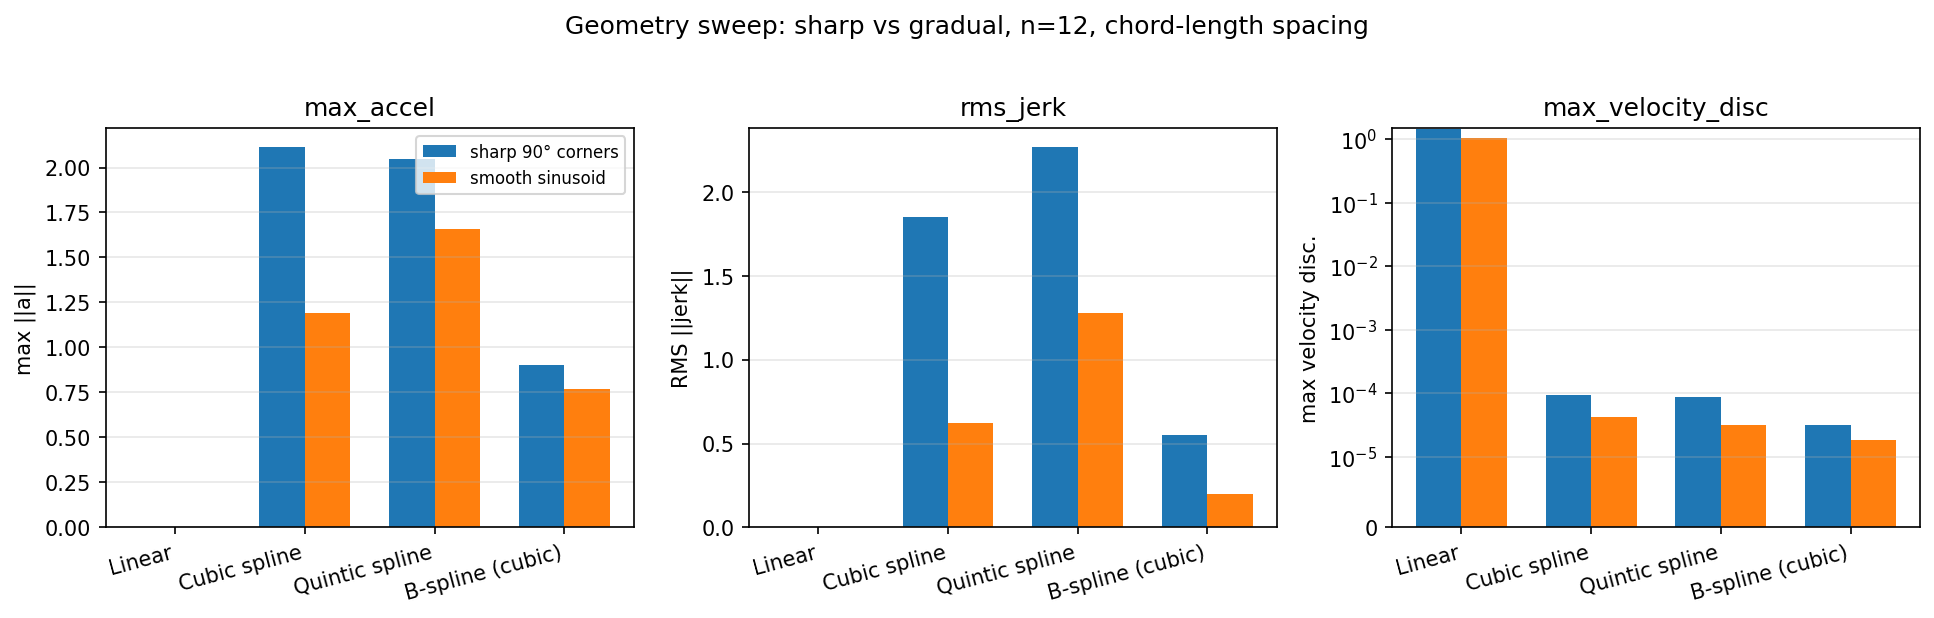
\includegraphics[width=\linewidth]{sweep_geometry.png}
\caption{Geometry sweep at $n=12$: sharp 90$^{\circ}$ zigzag versus
smooth sinusoid. The third panel uses a symmetric-log scale and
cleanly separates the linear interpolant ($\sim 1$\,m/s real
velocity discontinuity) from the smooth methods ($\sim 10^{-5}$\,m/s).}
\label{fig:geometry-sweep}
\end{figure*}

The trajectory plots in \cref{fig:geometry-trajectories} show why.
On the sharp zigzag, the cubic and quintic interpolants exhibit
Runge-style overshoot at every internal corner, attempting to
reconcile pass-through-every-waypoint with smooth derivatives. The
B-spline does not overshoot but cuts each corner aggressively, with
correspondingly small derivative magnitudes. On the smooth sinusoid,
all three smooth methods agree closely.

\begin{figure*}[!t]
\centering
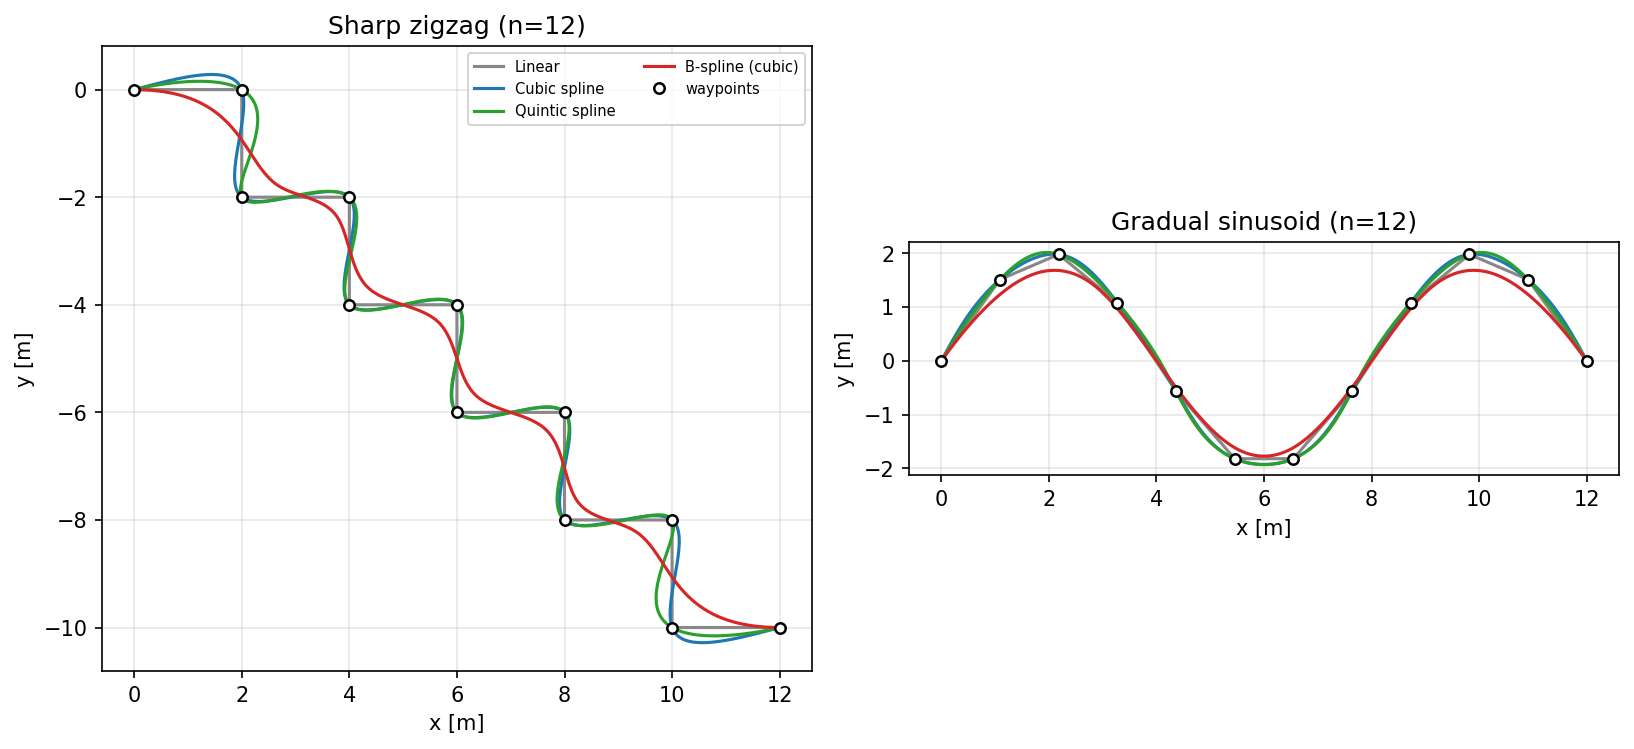
\includegraphics[width=\linewidth]{sweep_geometry_trajectories.png}
\caption{Mobile-robot trajectories on the sharp zigzag (left) and
gradual sinusoid (right) variants at $n=12$. Cubic and quintic
splines overshoot at sharp corners; the B-spline cuts them.}
\label{fig:geometry-trajectories}
\end{figure*}

\subsection{Spacing sweep}
\label{sec:results-spacing}

The third axis is the smallest in magnitude
(\cref{fig:spacing-sweep}). Switching from chord-length to uniform
time spacing on the same 12-waypoint mixed geometry leaves peak
acceleration and RMS jerk within roughly 30\% across all methods.
The most visible effect is on peak speed: the linear interpolant's
chord-length-parameterised speed envelope is identically 1\,m/s, but
under uniform spacing it must traverse the long diagonal segments in
the same one-second budget as the short ones, pushing peak speed to
1.32\,m/s. The smooth methods inherit some of this effect to a
lesser degree.

\begin{figure*}[!t]
\centering
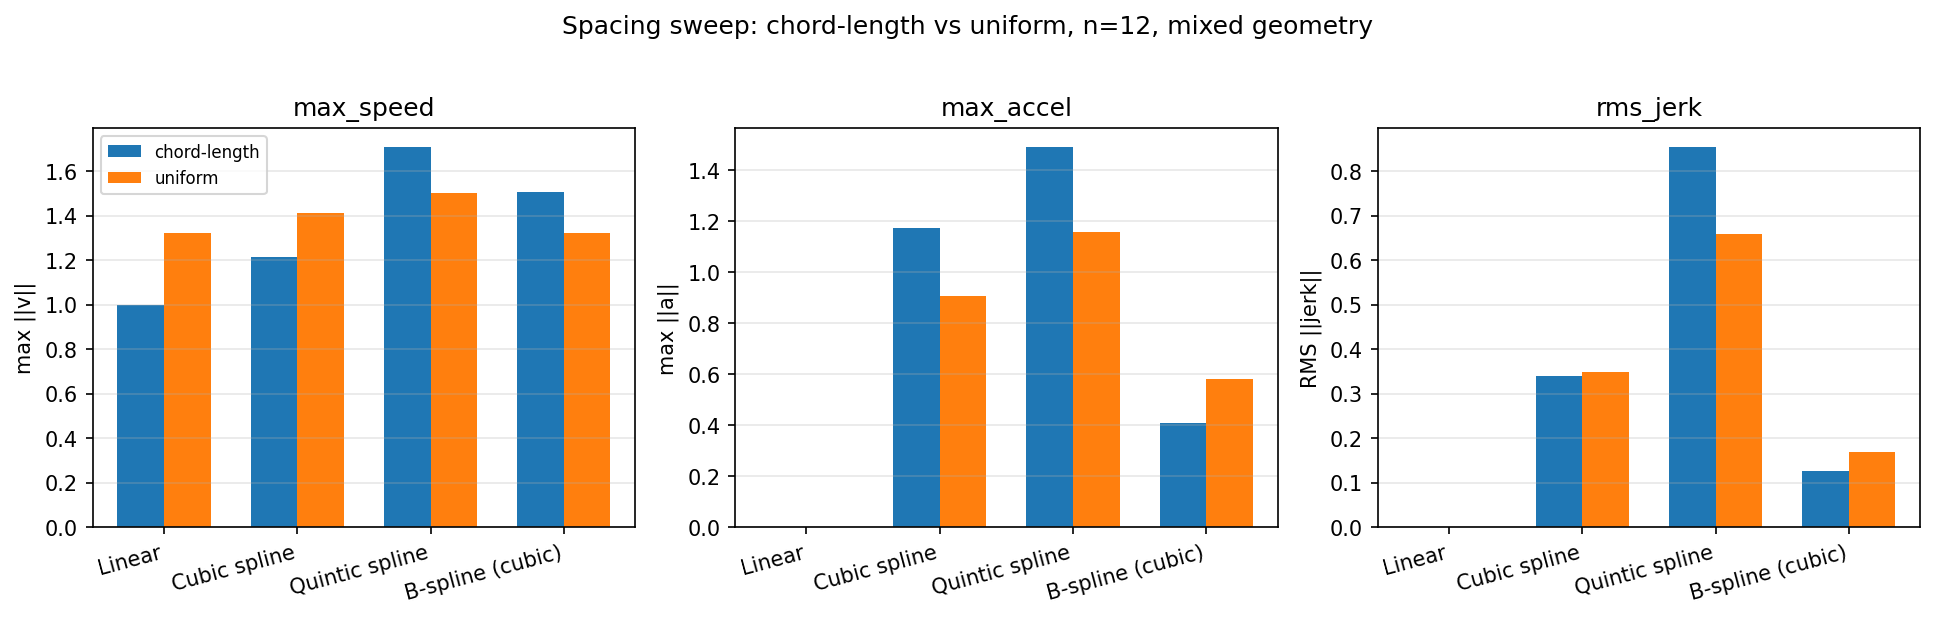
\includegraphics[width=\linewidth]{sweep_spacing.png}
\caption{Spacing sweep: chord-length versus uniform time spacing at
$n=12$ on the mixed geometry. Peak speed is the most affected
metric; peak acceleration and RMS jerk are within 30\%.}
\label{fig:spacing-sweep}
\end{figure*}

\subsection{Derivative validation}
\label{sec:results-validation}

\Cref{fig:validation} compares each method's analytic derivative
output against centered finite-difference estimates of the same
underlying dense position trajectory, using the schemes from
Section~\ref{sec:bg-diff} on the cubic spline run. The two curves
overlap to plotting precision in the velocity and acceleration
panels. The jerk panel shows the only meaningful disagreement: the
cubic spline has true step discontinuities in jerk at every internal
knot, and the centered five-point finite-difference scheme cannot
resolve those steps, instead smoothing each into a short ramp.

\begin{figure*}[!t]
\centering
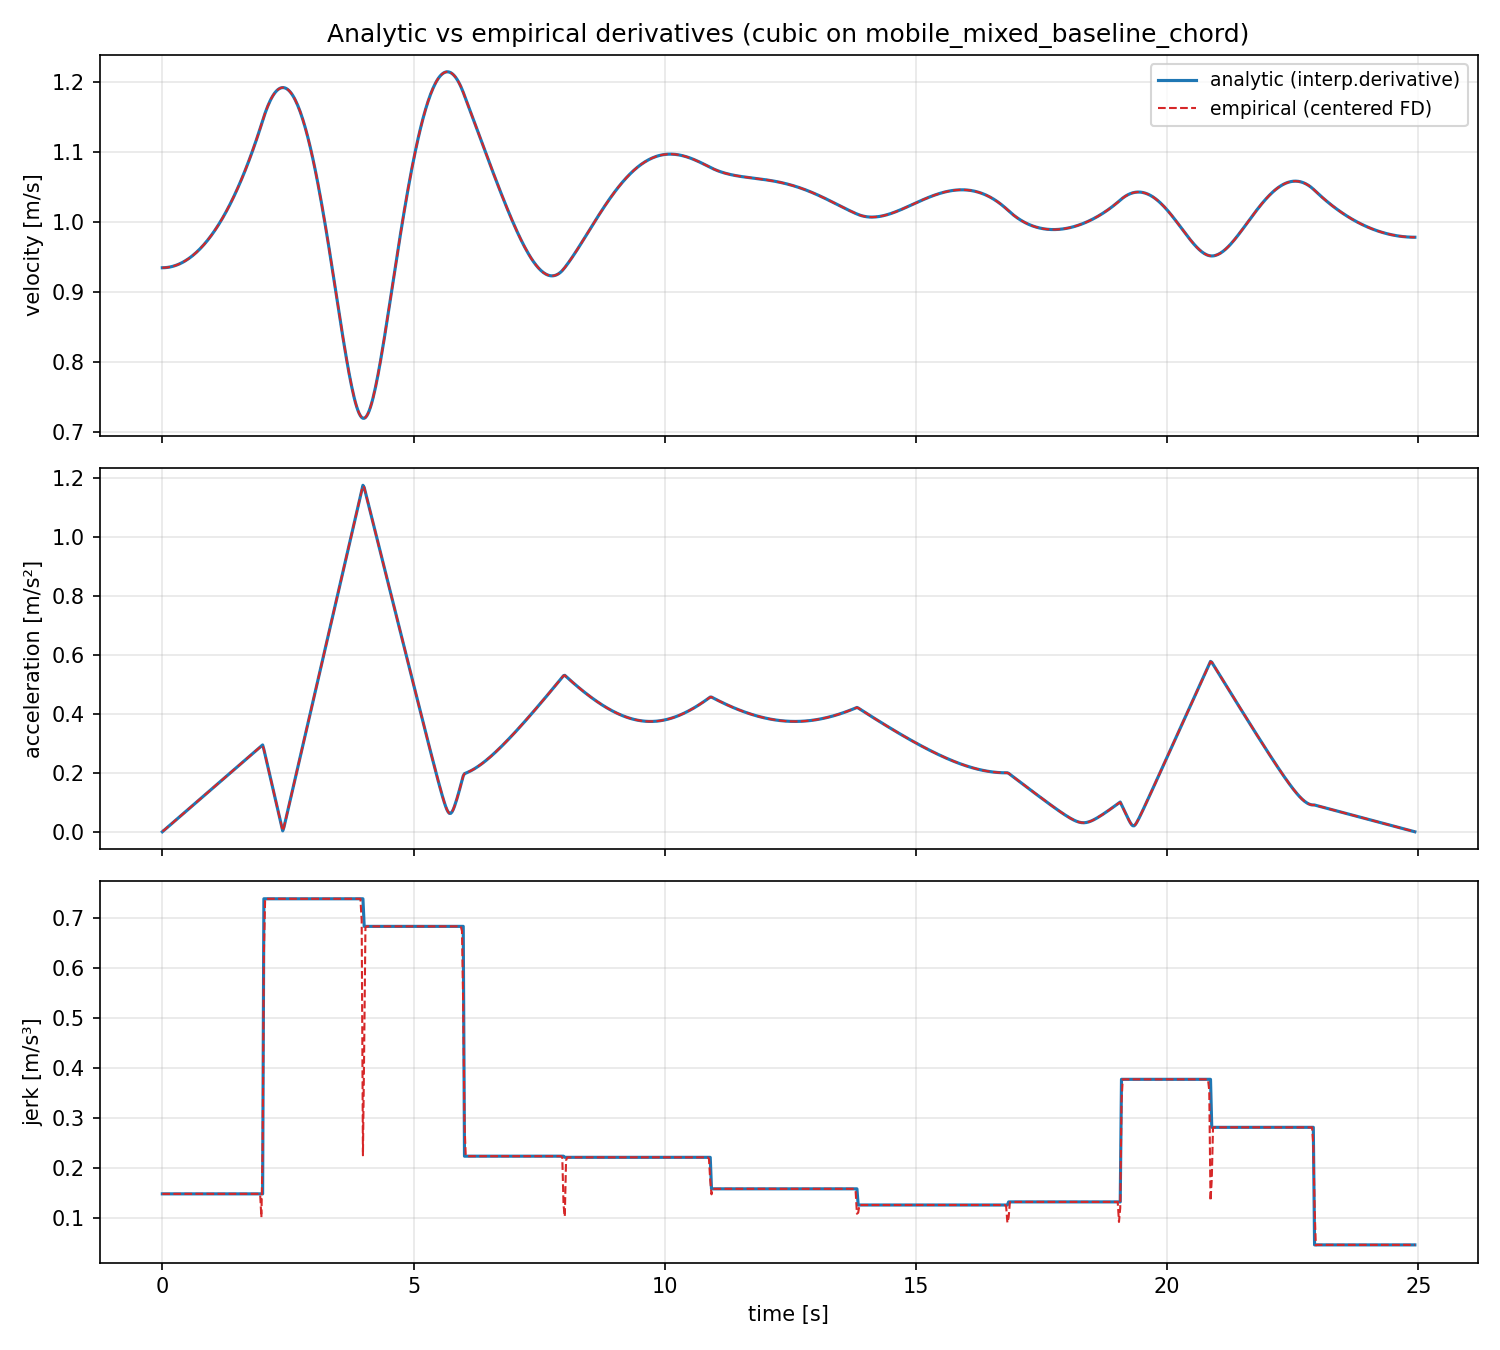
\includegraphics[width=0.78\linewidth]{validation_analytic_vs_empirical.png}
\caption{Analytic derivative vs.\ centered finite-difference
empirical derivative for the cubic spline on the baseline mobile
robot. Velocity and acceleration overlap to plotting precision; the
jerk panel shows the FD scheme's expected smoothing of the
analytic step discontinuities at internal knots.}
\label{fig:validation}
\end{figure*}

The maximum interior errors are summarised in
\cref{tab:validation-errors}. The cubic-spline jerk error is
several orders of magnitude larger than the velocity or acceleration
errors because the latter are smooth functions of the cubic
polynomial pieces while the former is genuinely discontinuous. The
quintic and B-spline jerk errors are at the $10^{-3}$ to $10^{-1}$
level, consistent with their respective continuity classes.

\begin{table}[!t]
\centering
\caption{Maximum interior errors of analytic vs.\ finite-difference
derivatives, baseline mobile-robot dataset. Boundary stencils are
excluded from the comparison.}
\label{tab:validation-errors}
\begin{tabular}{lccc}
\toprule
\textbf{Method} & $\max |v_a - v_e|$ & $\max |a_a - a_e|$ & $\max |j_a - j_e|$ \\
\midrule
Cubic    & $2.6 \times 10^{-5}$ & $2.3 \times 10^{-3}$ & $5.1 \times 10^{-1}$ \\
Quintic  & $7.3 \times 10^{-8}$ & $4.3 \times 10^{-4}$ & $8.8 \times 10^{-4}$ \\
B-spline & $5.1 \times 10^{-6}$ & $6.6 \times 10^{-4}$ & $1.3 \times 10^{-1}$ \\
\bottomrule
\end{tabular}
\end{table}

\subsection{Quintic boundary-condition sensitivity}
\label{sec:results-bc-sens}

The boundary-condition sensitivity study
(Section~\ref{sec:bc-sensitivity-method}) identifies the natural BC
as the source of the quintic spline's anomalously high derivative
norms (\cref{fig:quintic-bc}). Replacing the natural BC
($\vec{v}_0 = \vec{a}_0 = \vec{v}_n = \vec{a}_n = \vec{0}$) with the
cubic-derived clamped BC reduces peak acceleration from
1.49\,m/s$^2$ to 1.00\,m/s$^2$ (a 33\% reduction) and RMS jerk from
0.85\,m/s$^3$ to 0.31\,m/s$^3$ (a 64\% reduction).

\begin{figure*}[!t]
\centering
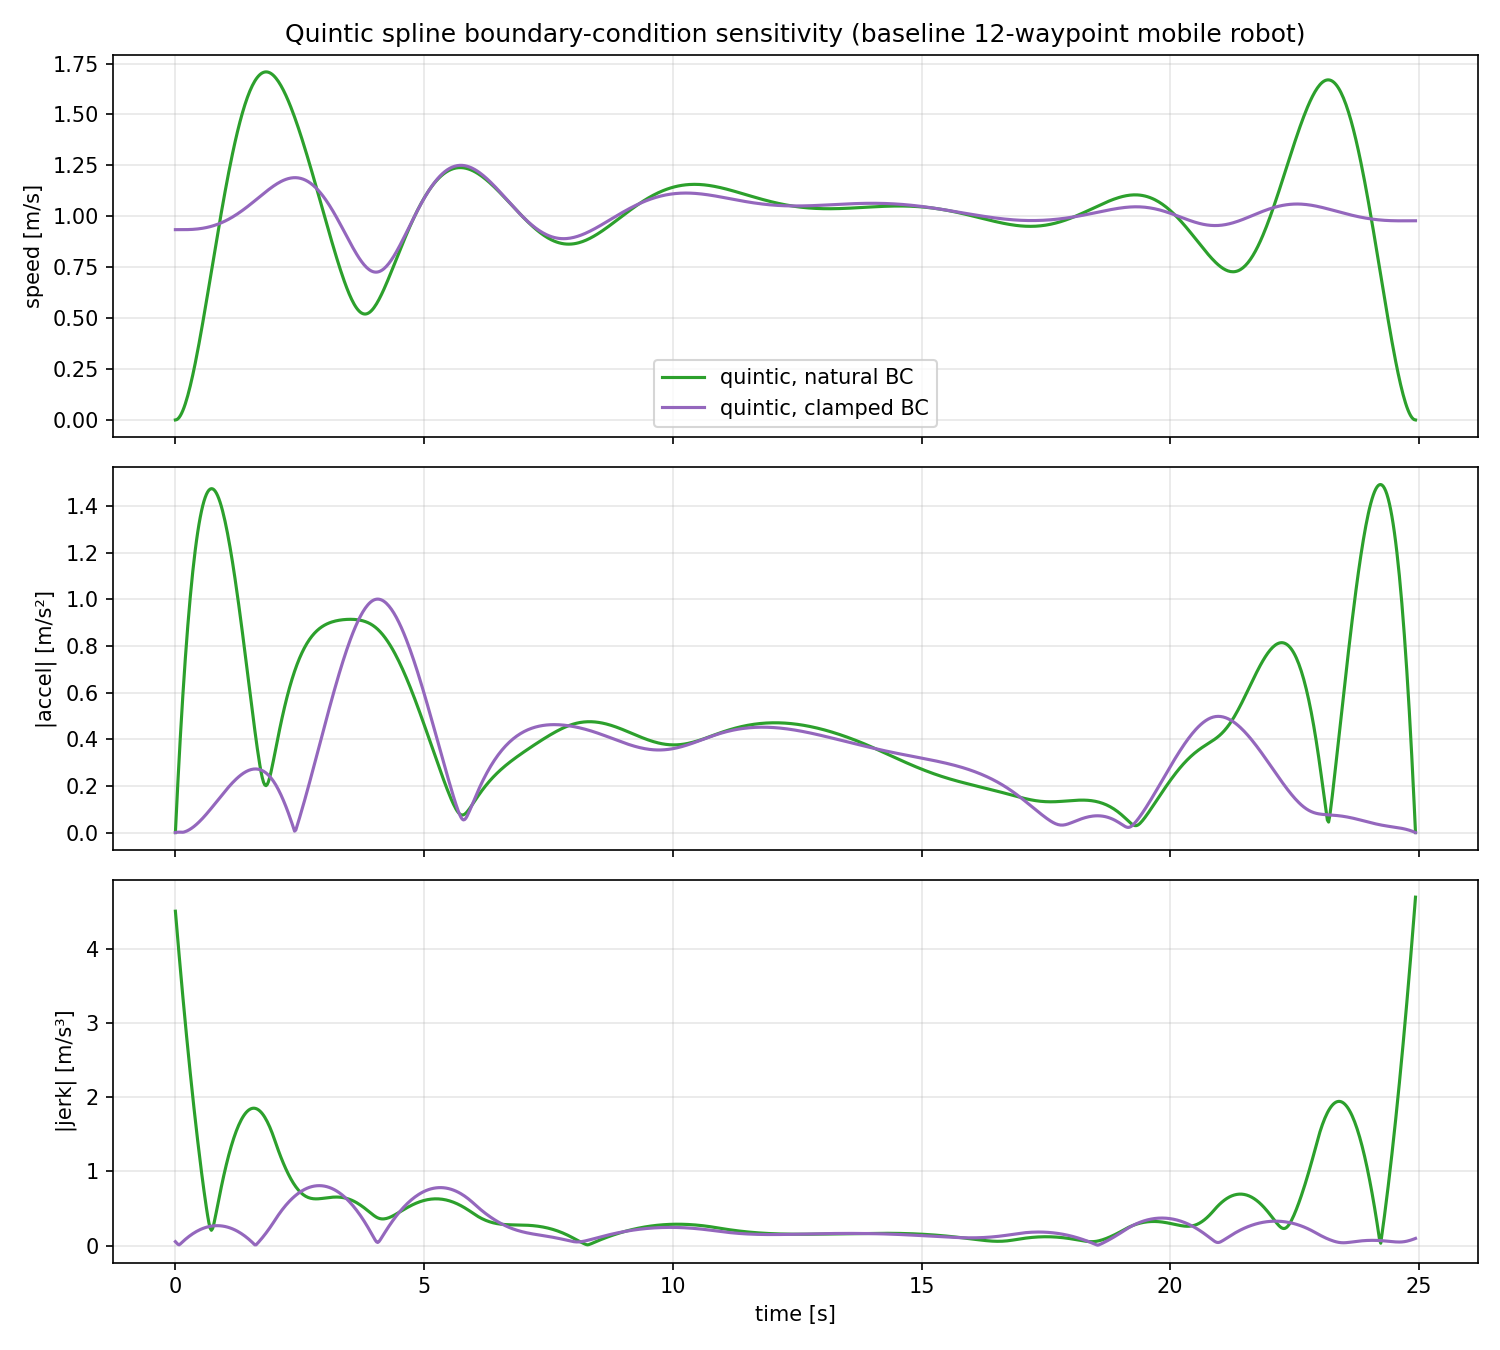
\includegraphics[width=0.78\linewidth]{quintic_bc_sensitivity.png}
\caption{Quintic spline boundary-condition sensitivity, mobile-robot
baseline. Natural BC forces start/stop-at-rest in both velocity and
acceleration, generating large endpoint-region jerk. Clamped BC
with cubic-derived end-velocities and end-accelerations removes the
endpoint spikes entirely.}
\label{fig:quintic-bc}
\end{figure*}

With the cubic-derived clamped BC, the quintic is the smoothest
interpolating method on the baseline---outperforming the cubic on
every metric except peak velocity. The natural-BC quintic should
therefore be reported as a method-plus-BC choice in published
results, not as an inherent property of quintic splines.


% =====================================================================
% Discussion
% =====================================================================
\section{Discussion}
\label{sec:discussion}

We organise the discussion around eight findings supported by the
data in Section~\ref{sec:results}.

\subsection{Waypoint adherence is a hard distinction, not a continuum}
\label{sec:disc-waypoint}

Linear, cubic, and quintic splines hit every waypoint to
floating-point precision on every variant in the experimental sweep,
while the B-spline approximation deviates by 0.28--0.92\,m on the
mobile-robot variants and 0.40\,rad on the robot arm. Increasing
waypoint density does not eliminate this deviation, because the
B-spline's clamped knot vector forces interpolation only at the
endpoints; the interior of the curve is fundamentally an
\emph{approximation} of the input control polygon. This is the
defining trade-off of the formulation, not a tuning parameter.

For applications in which the waypoints are strict constraints
(picking a part at an exact location), a B-spline approximation is
inappropriate regardless of how smooth its derivatives may be. For
applications in which the waypoints are soft guidelines (smoothing a
collision-avoidance buffer), the trade-off may be acceptable or even
desirable.

\subsection{Linear interpolation is the only method with $C^1$
violations}
\label{sec:disc-linear-c1}

The \texttt{max\_velocity\_disc} column quantifies $C^1$ violation
directly: linear interpolation produces $\sim 1$\,m/s velocity
discontinuities at every waypoint regardless of geometry, while the
smooth methods sit at or below $10^{-4}$\,m/s---essentially
numerical noise. The standard ``zero acceleration / zero jerk'' rows
of the linear results in \cref{tab:baseline-metrics} are therefore
misleading: they characterise the analytic derivative on the open
intervals between waypoints, not the distributional sense in which
the second derivative contains Dirac impulses.

A controller that finite-differences the commanded position, as is
standard in cascade-controlled servomechanisms, would observe
acceleration spikes proportional to its sampling rate at every
waypoint. The mismatch between the analytic and physical
interpretation of the linear-interpolation metrics motivates
reporting \texttt{max\_velocity\_disc} alongside the other metrics
in any future study.

\subsection{Adding waypoints can worsen smoothness}
\label{sec:disc-density}

The density sweep results
(Section~\ref{sec:results-density}) show that on the mixed geometry
under chord-length parameterisation, peak acceleration and RMS jerk
both increase monotonically with waypoint count for every spline
method. The mechanism is direct: chord-length parameterisation keeps
each segment's nominal speed at 1\,m/s, so denser waypoints reduce
$h_i$ proportionally. Because spline curvature scales like
$1/h_i^2$ and jerk like $1/h_i^3$, denser inputs force larger time
derivatives.

This finding contradicts the naive intuition that more waypoints
always means smoother motion. The correct interpretation is that
denser waypoints buy \emph{geometric fidelity}---the trajectory
converges towards the polyline as $n$ grows---at the price of
larger time-derivative magnitudes. Practitioners should choose
waypoint density based on which property matters more in their
application, not on the assumption that one trade-off dominates.

\subsection{Geometry dominates the smoothness budget}
\label{sec:disc-geometry}

Switching from a smooth sinusoid to a sharp 90$^{\circ}$ zigzag at
fixed $n=12$ approximately doubles peak acceleration and triples RMS
jerk for cubic and quintic splines---a much larger effect than any
of the other axes we tested. Geometry is therefore the dominant
determinant of how aggressively each method has to bend.

The B-spline absorbs this geometric character much more gracefully
than the interpolating splines: its sharp-vs.-gradual peak
acceleration ratio is only 1.18, compared to 1.78 for the cubic and
1.24 for the natural-BC quintic. This is a direct consequence of the
B-spline's approximation property---it is allowed to soften the
corner---and explains why B-splines are preferred in trajectory
planning for paths with intentionally sharp features such as
obstacle avoidance.

\subsection{Time spacing matters less than expected}
\label{sec:disc-spacing}

The textbook recommendation to use chord-length parameterisation
\cite[Section 24.1]{chapra2021} is reasonable but not as critical as
density or geometry. Switching to uniform spacing on the same
12-waypoint mixed geometry leaves peak acceleration and RMS jerk
within $\sim 30\%$ across all methods. The most visible effect is on
peak speed under linear interpolation, where uniform spacing forces
the robot to traverse long diagonals in the same time as short
straight segments.

For practical use, chord-length parameterisation remains the
default but the penalty of uniform spacing is modest enough that
implementers facing constraints (such as fixed-rate trajectory
buffers) need not feel obligated to enforce it.

\subsection{The quintic spline's apparent inferiority is a
boundary-condition artefact}
\label{sec:disc-quintic-bc}

The most surprising result in the baseline study is that the quintic
spline produced higher peak acceleration and RMS jerk than the cubic
on both datasets despite its higher continuity class
(\cref{tab:baseline-metrics}). The boundary-condition sensitivity
study (Section~\ref{sec:results-bc-sens}) explains this anomaly:
under natural BC the quintic must start and stop at rest in both
velocity and acceleration, but the rest of the spline is fitted to a
chord-length parameterisation that implies a 1\,m/s nominal speed;
reconciling these two demands within the first and last segment
forces a rapid transition with $\sim 4.5$\,m/s$^3$ jerk spikes at the
endpoints.

Replacing the natural BC with cubic-derived clamped BC---reading
$v_0$, $v_n$, $a_0$, $a_n$ off the cubic spline solution and
applying them as quintic boundary values---reduces peak acceleration
by 33\% and RMS jerk by 64\%, making the clamped quintic the
smoothest of the three interpolating methods on this dataset.

The practical implication is twofold. First, published comparisons
of quintic splines should explicitly state the boundary condition,
not just the method. Second, for applications where end velocities
and accelerations are known (a robot moving from one continuous
trajectory to another), the clamped quintic is the recommended
choice.

\subsection{Analytic derivatives match numerical differentiation}
\label{sec:disc-validation}

Centered finite-difference estimates of the dense-sampled trajectory
agree with the analytic derivatives to better than $10^{-3}$\,m/s$^2$
for acceleration and $10^{-3}$\,m/s$^3$ for jerk on the cubic,
quintic, and B-spline interpolants. This validates the textbook
analytic formulas of Section~\ref{sec:bg-cubic}--\ref{sec:bg-bspline}
as correct for the intended use.

The single exception---cubic spline jerk, with $5.1 \times 10^{-1}$
error---is not an implementation bug. The cubic spline's jerk is a
piecewise constant function with step discontinuities at every
internal knot. The five-point centered finite-difference scheme
cannot resolve those steps and instead smooths each into a ramp of
width $\sim 5h$. The error magnitude reflects the height of the
worst step in the dataset, not any error in the analytic formula.

\subsection{Computational cost is not a deciding factor}
\label{sec:disc-compute}

Even the most expensive method (the quintic, which solves a dense
$2(n+1) \times 2(n+1)$ linear system before evaluating) finishes in
under one millisecond at every density studied, including dense
evaluation at 1000 sample points. The full 28-row experiment runs
end-to-end in approximately 30\,ms.

For the problem sizes typical of robotic trajectory generation
(tens to low hundreds of waypoints), computation time is not a
deciding factor. The interesting trade-offs are between waypoint
adherence, smoothness, and geometric fidelity, not between methods
of different asymptotic cost.


% =====================================================================
% Conclusion
% =====================================================================
\section{Conclusion}
\label{sec:conclusion}

We have presented a comparative analysis of four numerical
interpolation methods drawn from Chapters~18 and~24 of Chapra and
Canale---linear interpolation, natural cubic splines, $C^4$ quintic
Hermite splines, and cubic B-spline approximation---applied to the
problem of robot trajectory generation. Every method was implemented
directly from the textbook formulation, validated against reference
implementations and analytic test functions, and exercised on two
realistic robotics scenarios sweeping over waypoint density,
geometric character, and time spacing.

The data support eight findings (Section~\ref{sec:discussion}), of
which three are non-obvious and worth re-emphasising. \emph{First},
adding waypoints under chord-length parameterisation \emph{worsens}
smoothness metrics for spline methods, despite the popular intuition
that more data is always better. \emph{Second}, the quintic spline
under natural boundary conditions produces \emph{higher} peak
acceleration and RMS jerk than the cubic on both datasets---an
artefact entirely attributable to the boundary condition rather
than the method, since cubic-derived clamped boundary conditions
reduce peak acceleration by 33\% and RMS jerk by 64\%.
\emph{Third}, the cubic B-spline absorbs sharp input geometry much
more gracefully than the interpolating splines, at the cost of a
guaranteed 0.28--0.92\,m waypoint deviation in our scenarios.

\subsection{Recommendations}
\label{sec:recommendations}

Based on the analysis, we recommend the following decision rule for
practitioners choosing among these methods:

\begin{itemize}[leftmargin=*]
\item If waypoints are strict constraints and the application has
known end-velocities and end-accelerations (e.g.\ stitching together
pre-planned segments), use a \textbf{clamped quintic spline}; this
configuration combines exact waypoint adherence with $C^4$
continuity and the smoothest derivative norms in our experiments.
\item If waypoints are strict constraints but the system is expected
to start and stop at rest with no other prior information, use a
\textbf{natural cubic spline}; the natural-BC quintic should be
avoided because of the endpoint jerk spike documented in
Section~\ref{sec:results-bc-sens}.
\item If waypoints are soft guidelines and the path contains
intentionally sharp geometric features (e.g.\ obstacle-avoidance
clearances), a \textbf{cubic B-spline approximation} is preferred for
its substantially smoother derivative profile.
\item Linear interpolation is appropriate only as a baseline or for
debugging; it should not be deployed without an additional
post-processing smoothing step because of the velocity discontinuity
at every waypoint.
\end{itemize}

\subsection{Limitations}
\label{sec:limitations}

The study has several limitations that constrain the generality of
the conclusions.

The datasets are synthetic. Real industrial waypoint sequences come
from path planners with their own geometric biases, and the
distribution of inputs in deployed systems may differ from our
constructed mixed/sharp/gradual variants. Replicating the analysis
on a corpus of real recorded trajectories would strengthen the
external validity of the findings.

The metrics are kinematic only. We do not include actuator-saturation
limits, mechanical resonance frequencies, payload disturbance
models, or thermal limits, all of which are relevant to trajectory
quality in deployed systems and could be incorporated into a
weighted composite metric.

Only two boundary-condition variants of the quintic spline are
explored. A more thorough sensitivity study would sweep over a
range of clamped end-velocities and end-accelerations, or
investigate alternative boundary specifications such as periodic or
not-a-knot conditions.

\subsection{Future work}
\label{sec:future-work}

Several extensions of this work are natural follow-ups for
Deliverable~4 or beyond:

\begin{enumerate}[leftmargin=*]
\item \textbf{Optimised B-splines.} The B-spline approximation has
free parameters in the choice of knot vector and the placement of
control points; a constrained optimisation that minimises waypoint
deviation while preserving smoothness would close the
waypoint-fidelity gap.
\item \textbf{Time-optimal reparameterisation.} The current study
fixes the time parameterisation a priori. Methods such as
time-scaling under acceleration or jerk constraints
\cite{macfarlane2003jerk} would let each method run at its physical
limit, providing a fairer comparison across methods.
\item \textbf{High-dimensional configuration spaces.} The 2-DOF arm
is the simplest non-trivial manipulator. Repeating the analysis on
a 6-DOF or 7-DOF arm would test whether the findings generalise.
\item \textbf{Comparison with geometrically-aware methods.} Methods
such as PH curves and minimum-jerk trajectories
\cite{kyriakopoulos1988minimum} provide alternatives that the
classical interpolation methods compared here do not, and a head-to-
head comparison would situate our results within the broader
trajectory-planning literature.
\end{enumerate}

\subsection{Reproducibility}

All code, datasets, and results are available in the project
repository, including:

\begin{itemize}[leftmargin=*]
\item Python implementations of all four interpolation methods,
the centered finite-difference schemes from Chapter~28, and the
metric and visualisation utilities;
\item the canonical CSV waypoint datasets and the parametric variant
generators used to construct the experimental sweep;
\item an executable Jupyter notebook that regenerates every figure
and table in this paper from the raw data;
\item the complete experiment metric table
(\texttt{full\_experiment.csv}, 28 rows $\times$ 14 columns).
\end{itemize}

The full experiment runs in approximately 30\,ms on commodity
hardware, supporting independent re-derivation of every reported
result.


% ----- Bibliography ---------------------------------------------------
% IEEEtran bibliography style produces the canonical IEEE reference
% format, matching the .docx template.
\bibliographystyle{IEEEtran}
\bibliography{references}

\end{document}
